%%%%%%%%%%%%%%%%%%%%%%%%%%%%%%%%%%%%%%%%%%%%%%%%%%%%%%%%%%%%%%%%%%%%
% Grundlagen
%%%%%%%%%%%%%%%%%%%%%%%%%%%%%%%%%%%%%%%%%%%%%%%%%%%%%%%%%%%%%%%%%%%%

\chapter{Stand der Technik}
  \label{Stand der Technik}

\section{Beschreibung der Orientierung von Objekten im dreidimensionalen Raum}
Zur Beschreibung der Orientierung von Objekten im dreidimensionalen Raum in kartesischen Koordinatensystemen gibt es mehrere Möglichkeiten. Die drei am häufigsten verwendeten werden im Folgenden vorgestellt.

\subsection{Euler-Winkel}
Bei Euler-Winkeln handelt es sich um drei Winkel, die jeweils die Rotation um eine bestimmte Achse des Koordinatensystems angeben. So kann eine Transformation zwischen zwei Koordinatensystemen, dem Labor- und dem Körperfesten-System definiert werden.

Es existieren mehrere Definitionen von Euler-Winkeln, was die Reihenfolge der Drehungen um die Achsen anbelangt. Die bekannteste ist Yaw-Pitch-Roll - zu deutsch: Roll-Nick-Gier-Winkel. Dies entspricht auch der Luftfahrtnorm (DIN 9300).

\begin{itemize}
	\item Roll (Roll-Winkel) beschreibt die Querneigung, also die Drehung um die X-Achse.
	\item Pitch (Nick-Winkel) besschreibt die Längsneigung, also die Drehung um die Y-Achse.
	\item Yaw (Gier-Winkel) beschreibt Orientierung, also die Drehung um die Z-Achse.
\end{itemize}

Bei mobilen Geräten wie dem Apple iPhone, gibt es anders als bei Fahrzeugen, keine fest definierte Ausrichtung. Beim iPhone und iPad sind die Winkel darum so verteilt wie auf Abbildung \ref{fig:apple-axes} zu sehen.

\begin{figure}[htb]
\centering
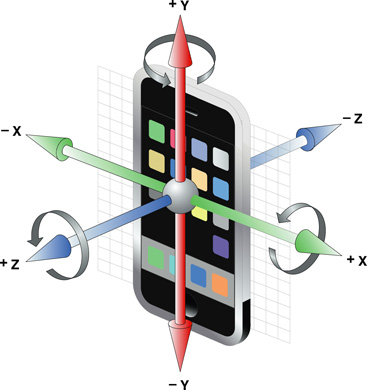
\includegraphics[scale=0.8]{figures/apple-axes}
\caption{Roll-Pitch-Yaw \cite{apple:001}}
\label{fig:apple-axes}
\end{figure}

Euler-Winkel haben den Vorteil, dass sie jeder intuitiv verstehen kann. Jeder lernt Euler-Winkel in der Schule kennen. Somit kann man mit ihnen auch einfach rechnen.

Eine Drehung mit Euler-Winkeln setzt sich immer aus einer Kombination von Rotation der drei Achsen zusammen. Das heißt, eine Drehung findet nie direkt statt, sondern über mehrere nacheinander ausgeführte Rotationen der einzelnen Achsen. Das kann bei manchen Anwendungen ein Problem sein. Zum Beispiel wenn die Orientierung schneller abgefragt wird als die Teilschritte einer Drehung berechnet werden, kann es vorkommen, dass in einzelnen Key-Frames der Anwendung falsche Orientierungsdaten einfließen.

Eine Orientierungs-Angabe als Euler-Winkel würde beispielsweise wie folgt aussehen: 
$$
\begin{pmatrix}
    \alpha\\ 
    \beta\\ 
    \gamma
  \end{pmatrix} =
\begin{pmatrix}
    0.016134\\ 
    -0.000284\\ 
    1.618407
  \end{pmatrix} 
$$
Die Werte sind in Radiant angeben. Negative Werte können zustande kommen, da die Skala von $-\pi$ bis $+\pi$ geht.

\subsubsection{Gimbal Lock}
Der große Nachteil von Euler-Winkeln ist der Gimbal Lock (engl. f. Blockade der Kardanischen Aufhängung). So nennt man es wenn zwei Achsen die selbe Drehung bestimmen. Dadurch fehlt ein Freiheitsgrad. Man kann eine bestimmte Drehung erst dann wieder durchführen, wenn man eine der beiden zusammengefallenen Achsen zurück dreht. In Abbildung \ref{fig:gimbal-lock} ist leicht zu erkennen, dass die innere (blau) und äußere (grün) Achse die selbe Drehung bestimmen. Es ist daher momentan nicht möglich, das Flugzeug nach vorne oder hinten zu kippen. Zuerst müsste das Flugzeug entlang der mittleren Achse um $90^o$ gedreht werden. \cite{ paper:001}

\begin{figure}[htb]
\centering
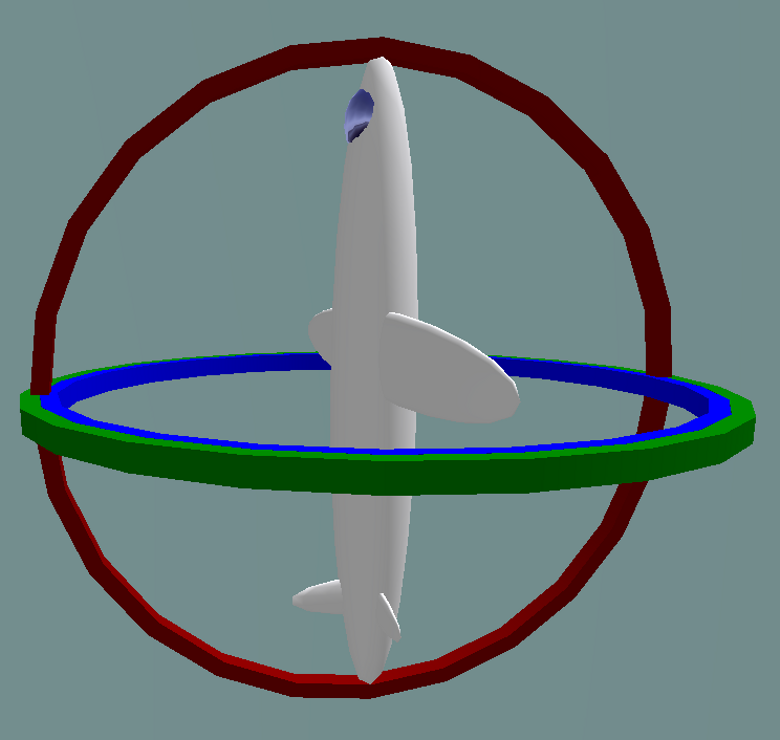
\includegraphics[scale=0.4]{figures/gimbal-lock}
\caption{Gimbal Lock \cite{ wiki:004} }
\label{fig:gimbal-lock}
\end{figure}

\subsection{Rotationsmatrizen}
Eine Rotationsmatrix ist eine orthogonale Matrix, die ebenfalls die Drehung im Raum beschreibt. Sie ist als eine Hintereinanderausführung einer oder mehrerer Rotationen um beliebige Drehachsen im dreidimensionalen Raum definiert. Rotationsmatrizen sind also eine Zusammenfassung von einzelnen Rotationen mit Euler-Winkeln in ein einziges Konstrukt. Gimbal Lock kann auch mit Rotationsmatrizen auftreten. \cite{ wiki:003}

Diese Rotationsmatrix entspricht einer Drehung um die x-Achse.
$$
R_x(\alpha) = \begin{pmatrix} 
1 &   0         & 0           \\
0 & \cos \alpha & -\sin \alpha \\
0 & \sin \alpha &  \cos \alpha
\end{pmatrix} 
$$

\subsection{Quaternionen}
Quaternionen sind ein mathematisches Konstrukt, um Orientierung von Objekten im dreidimensionalen Raum zu beschreiben. Sie setzen sich aus einem skalaren und einem vektoriellen Teil zusammen. Der vektorielle Teil ist allein dazu da, um die Achse der durchzuführenden Drehung zu beschreiben. Der Skalaranteil gibt den Winkel der Drehung an. Es wird also für jede Rotation eine eigene Achse konstruiert entlang der gedreht wird. Dadurch gibt es keine Zwischenschritte, sondern nur eine einzige Rotation. So kann auch das Problem des Gimbal Locks garnicht erst entstehen.

$$
q=\left\lbrack
0.056036\cdot \begin{pmatrix}
0.013658\\
-0.980339\\
0.188705
\end{pmatrix}\right\rbrack
= \left\lbrack w\cdot\begin{pmatrix}
x\\
y\\
z
\end{pmatrix} \right\rbrack
$$
Ein Quaternion sieht zum Beispiel so aus, wobei $w$ der oben angesprochene skalare Teil ist. \cite{paper:001}


\section{Positionsbestimmung}
Die Positionsbestimmung erfolgt in diesem Fall über Bluetooth. Dazu werden in dem Raum, in dem man navigieren möchte, Bluetooth-Sender (Beacons) ausgelegt. Diese sollten möglichst gleichmäßig verteilt sein, damit eine gleichmäßige Bluetooth-Abdeckung gewährleistet ist. Die App weiß, wo sich die einzelnen Beacons im Raum befinden und empfängt die RSSI-Werte der ausgelegten Beacons und kann so die Position des Geräts bestimmen. 

Dabei können mehrere Probleme auftreten. Das größte ist die Senderate der Beacons. Herkömmliche Bluetooth-Sticks sind dafür gemacht, eine ständige Verbindung zu einem Gerät aufrechtzuerhalten um Daten zu übertragen. Hier sollen keine Daten übertragen werden, sondern nur möglichst oft der RSSI-Wert der einzelnen Beacons erfahren werden. Normale Bluetooth-Sticks schaffen meistens nur eine Rate von ca. drei Sekunden. Das ist zu wenig um mit wenigen Sticks eine zuverlässige Navigation zu realisieren. Man muss entweder in relativ teure (über 100\texteuro) Bluetooth-Sender investieren die schnell sind, oder viele von den langsameren Sendern auslegen.

Ein weiteres Problem ist, dass Bluetooth leicht gestört werden kann. Personen, Wände und Bücherregale sind ein Problem bei Bluetooth. Darum kann man nicht sicher sein, dass die RSSI-Werte, die beim Gerät ankommen, die entsprechende Entfernung repräsentieren. 

Um diesen beiden Hauptproblemen entgegenzuwirken, wird ein Partikelfilter eingesetzt. Mit dem Partikelfilter wird eine Wolke gewichteter Partikel erzeugt, die den aktuellen Aufenthaltsort schätzt. Anhand der aktuellsten Position, die aus den Bluetooth-RSSI-Werten berechnet wurde, werden die einzelnen Partikel gewichtet. So kann die Ungenauigkeit der Bluetooth-Werte etwas korrigiert werden. \cite{wiki:001}